%for testing sectioning purpose
% \section{Test thu}
% \input{chapters/sections/sections2.1

\section{Microcontroller}
  \subsection{Theory}
  \gls{mcu} is a small size, special purpose computer. It is small enough in order to be integrated on a small circuit in which will do specified tasks or applications. MCU itself comes with memory, input, output peripherals and processor. Program to run the MCU is stored in \gls{rom} and usually not change in production. A microcontroller is usually designed to run in small size and at low cost, which is compatible to be embedded in other system in order to control actions of the system automatically.

  Few advantages of \gls{mcu} over a microprocessor can be listed as following:
  \begin{itemize}
    \item A MCU is already a standalone microcomputer.
    \item Because it can be considered as an independent computer, most needed components are integrated on a small size board.
    \item The above reason leads to the benefit that using MCU can make the system compact, highly mobile and cost efficiency.
    \item Time reduction because it is programed to run specified set of commands only.
    \item It is also easy to use and maintain.
    \item MCU nowadays usually designed to be used with low power in order to last longer under energy-limited condition.
  \end{itemize}

  \subsection{Microcontroller structure}
  Figure~\ref{fig:mcuStructure} demonstrates the basic structure of a microcontroller. It is easily to see the basic design of a microcontroller and its components.
  \begin{figure}[!ht]
    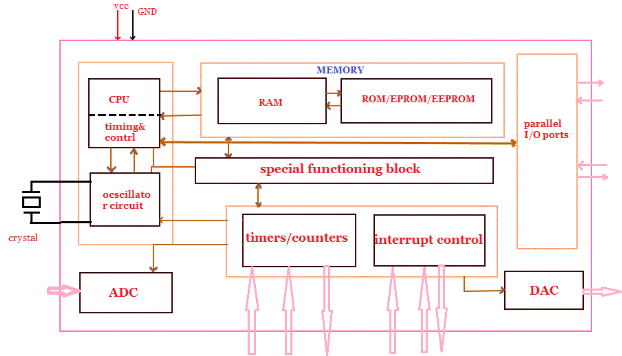
\includegraphics[scale=0.9]{images/Microcontroller-Structure.png}
    \caption{Structure of Microcontroller}
    \label{fig:mcuStructure}
  \end{figure}
  
  \begin{itemize}
    \item CPU: is the central unit which is assembled with \gls{alu} and a \gls{cu}. Its functions are connect parts of the MCU into a single system by doing fetch, decode and execution.
    \item Memory: there are two types of Memory that are required, namely \gls{rom} and \gls{ram}. Each type has its own functions, in which ROM will handle the program and the written instructions and RAM can only store temporary data while the program is executing.
    \item Input/Output: the single board system needs input to execute the program as well as outputs to delivery the information for further handling. The I/O peripherals are the interface of the MCU to communicate with or to control other devices.
    \item Bus: bus is the system of wires that used to connect the \gls{cpu} with other peripherals, which means it plays an important role but rarely discussed.
    \item Timers/Counters: they are built-in components for microcontroller, which is used to count in order to handle external events.
    \item Interrupts: is used to interrupt that can be an external or internal one, which helps to execute an instruction(s) while the main program is executing. 
    \item ADC: \gls{adc}, its name says it all, which is a circuit use to convert analogs signal to digital signals. The reason to use ADC is most sensors available on the market can read only analog signal but CPU of the \gls{mcu} can read digital signal only, so a \gls{adc} is necessary for them to communicate.
    \item DAC: \gls{dac} similar to \gls{adc}, DAC is also a circuit which convert digital signals into analog signals for further processing.
  \end{itemize}


  \subsection{Microcontroller market}
  There exists many microcontrollers on the market which come in various sizes and capacities. The list is only containing very few popular MCU that the author knows of.
  \begin{itemize}
    \item Intel 8051
    \item STMicroelectronics STM8S (8-bit), ST10 (16-bit) and STM32 (32-bit)
    \item Atmel AVR (8-bit), AVR32 (32-bit), and AT91SAM (32-bit)
    \item Freescale ColdFire (32-bit) and S08 (8-bit)
    \item PIC (8-bit PIC16, PIC18, 16-bit dsPIC33 / PIC24)
    \item Renesas Electronics: RL78 16-bit MCU; RX 32-bit MCU; SuperH; V850 32-
    bit MCU; H8; R8C 16-bit MCU
    \item PSoC (Programmable System-on-Chip)
    \item Texas Instruments Microcontrollers MSP430 (16-bit), C2000 (32-bit), and
    Stellaris (32-bit)
  \end{itemize}

\section{Communication}
  \subsection{Introduction}
  Nowadays, there are various communication protocols can be used for the thesis, namely I2C, ISP, RS232, RS485, Bluetooth or Wi-Fi. Each protocol is designed to be suitable for specified purpose with different advantages or disadvantages, which means a perfect protocol does not exist. When making a decision to choose suitable protocols for the thesis, the trade-off between the stabilization and the speed of the communication protocol has been considered carefully.

  In this thesis, RS485 is chosen as the main way for components in the system to communicate with each other. RS485 is defined in 1983 not as a protocol but an electrical interface standard and only specifies the drivers and receivers’ characteristics. It is developed in order to make data rate and transmitting distance are inversely proportional. For instance, the data transmitting speed can reach 10 Mbps within distance of 16 meters or if the distance is extended to 1220 meters, the data rate is lower to 100 kbps. The advantage of RS485 over RS232, which is developed in 1960, is multiple nodes can be parallel connected to a bus. Additionally, the network can be extended in length and number of nodes easily by using simple connectors. Besides, Wi-Fi, Bluetooth, GSM and MQTT are also implemented in the thesis in order to take the advantages of different communication protocols in different circumstances. 
  
  \subsection{RS485 specifications}
  %rs485 highlight specs table
  Table shows the highlight specifications of RS485. With these specifications, RS485 was a robust interface standard and was able to meet the requirements in industries, in which implemented applications that need stable, fast and reliable connection. Figure~\ref{fig:fullHalfDuplex} demonstrates two ways to implement the connection with RS485, which are full-duplex and half-duplex. Full-duplex implementations require four-wire (two signal pairs) instead of two-wire in half-duplex implementations; But despite the downside of two-wire implementation is it is limited to half-duplex and needs attention to turn-around delay, in practical applications, half-duplex is most chosen. The reason is full-duplex solution depends on master-slave model, which means the slaves cannot communicate with each other. In modern designs of transceiver, the allowed number of nodes can connect to the bus is up to hundreds.
    %full-duplex, half-duplex implementation figure
    \begin{figure}[!ht]
      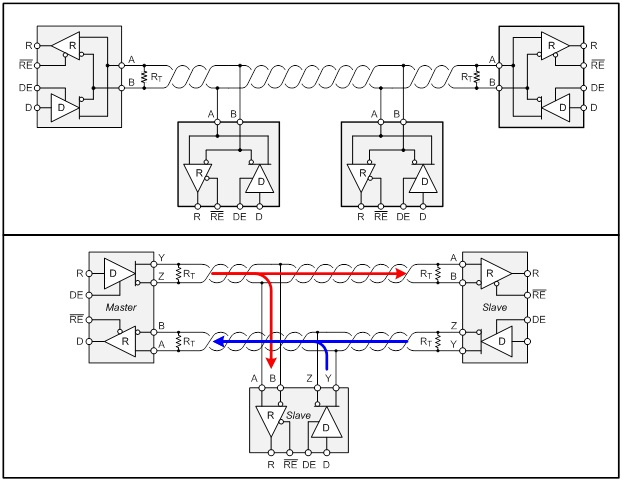
\includegraphics[scale=0.85]{images/rs485-fullduplex-halfduplex.jpg}
      \caption{Half-duplex(upper) and Full-duplex(below) implementations}
      \label{fig:fullHalfDuplex}
    \end{figure}


  


